\documentclass[xcolor=pdflatex,dvipsnames,table]{beamer}
\usepackage{epsfig,graphicx}
\usepackage{palatino}
\usepackage{fancybox}
\usepackage{relsize}
\usepackage[procnames]{listings}
\usepackage{hyperref}
\usepackage{qtree} % needed?
\usepackage{booktabs}
\usepackage{dirtree}
\usepackage[normalem]{ulem}


% fatter TT font
\renewcommand*\ttdefault{txtt}
% another TT, suggested by Alex
% \usepackage{inconsolata}
% \usepackage[T1]{fontenc} % needed as well?


\newcommand{\scale}{0.7}

\newcommand{\todo}[1]{{\emph{TODO: #1}}}
\newcommand{\martin}[1]{{\color{blue} Martin: #1}}
\newcommand{\abcdef}[1]{{\color{red} Author2: #1}}

% uncomment following for final submission
%\renewcommand{\todo}[1]{}
%\renewcommand{\martin}[1]{}
%\renewcommand{\author2}[1]{}

\newcommand{\code}[1]{{\texttt{#1}}}

\hypersetup{
  linkcolor  = black,
%  citecolor  = blue,
  urlcolor   = blue,
  colorlinks = true,
}

\beamertemplatenavigationsymbolsempty
\setbeamertemplate{footline}[frame number]





\newif\ifbook
% shared in slides and book

\lstdefinelanguage{chisel}{
  morekeywords={abstract,case,catch,class,def,%
    do,else,extends,false,final,finally,%
    for,if,implicit,import,match,mixin,%
    new,null,object,override,package,%
    private,protected,requires,return,sealed,%
    super,this,throw,trait,true,try,%
    type,val,var,while,with,yield},
  otherkeywords={=>,<-,<\%,<:,>:,\#,@},
  sensitive=true,
  morecomment=[l]{//},
  morecomment=[n]{/*}{*/},
  morestring=[b]",
  morestring=[b]',
  morestring=[b]"""
}

\usepackage{color}
\definecolor{dkgreen}{rgb}{0,0.6,0}
\definecolor{gray}{rgb}{0.5,0.5,0.5}
\definecolor{mauve}{rgb}{0.58,0,0.82}

% Default settings for code listings
\ifbook
\lstset{%frame=lines,
  language=chisel,
  aboveskip=3mm,
  belowskip=3mm,
  showstringspaces=false,
  columns=fixed, % basewidth=\mybasewidth,
  basicstyle={\small\ttfamily},
  numbers=none,
  numberstyle=\footnotesize,
  % identifierstyle=\color{red},
  breaklines=true,
  breakatwhitespace=true,
  procnamekeys={def, val, var, class, trait, object, extends},
  % procnamestyle=\ttfamily,
  tabsize=2,
  float
}
\else
\lstset{%frame=lines,
  language=chisel,
  aboveskip=3mm,
  belowskip=3mm,
  showstringspaces=false,
  columns=fixed, % basewidth=\mybasewidth,
  basicstyle={\small\ttfamily},
  numbers=none,
  numberstyle=\footnotesize\color{gray},
  % identifierstyle=\color{red},
  keywordstyle=\color{blue},
  commentstyle=\color{dkgreen},
  stringstyle=\color{mauve},
  breaklines=true,
  breakatwhitespace=true,
  procnamekeys={def, val, var, class, trait, object, extends},
  procnamestyle=\ttfamily\color{red},
  tabsize=2,
  float
}
\fi

\lstnewenvironment{chisel}[1][]
{\lstset{language=chisel,#1}}
{}

\newcommand{\shortlist}[1]{{\lstinputlisting[nolol]{#1}}}

\newcommand{\longlist}[3]{{\lstinputlisting[float, caption={#2}, label={#3}, frame=tb, captionpos=b]{#1}}}

\newcommand{\verylonglist}[3]{{\lstinputlisting[caption={#2}, label={#3}, frame=tb, captionpos=b]{#1}}}


\title{Testing and Verification}
\author{Martin Schoeberl}
\date{\today}
\institute{Technical University of Denmark\\
Embedded Systems Engineering}

\begin{document}

\begin{frame}
\titlepage
\end{frame}


\begin{frame}[fragile]{TODO}
\begin{itemize}
\item Midterm evaluation
\item \url{https://forms.gle/wtvDrA4peD4oLvt16}
\item Show ab solutions for last week
\item Show lab exercise 7-segment decoder
\item Also have the shift register (after some repetition)
\item  * link is missing: use simple bash scripts or Makefiles to remember commands (show examples)
\item Show CI of my book for testing, see also emails from Travis in jopdesign inbox
\end{itemize}
\end{frame}


\begin{frame}[fragile]{Generating Timing with Counters}
\begin{itemize}
\item Generate a \code{tick} at a lower frequency
\item E.g., used for driving the display multiplexing at 1~kHz
\end{itemize}
\begin{figure}
  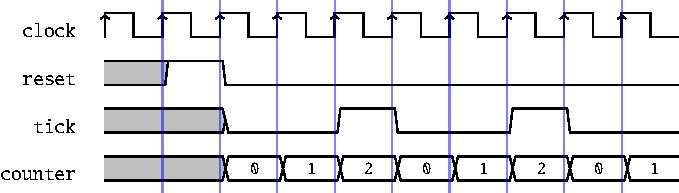
\includegraphics[scale=0.8]{../figures/tick_wave}
\end{figure}
\end{frame}


\begin{frame}[fragile]{The Tick Generation}
\shortlist{../code/sequ_tick_gen.txt}
\end{frame}

\begin{frame}[fragile]{Using the Tick}
\begin{itemize}
\item A counter running at a \emph{slower frequency}
\item By using the \code{tick} as an enable signal
\end{itemize}
\shortlist{../code/sequ_tick_counter.txt}
\end{frame}

\begin{frame}[fragile]{The \emph{Slow} Counter}
\begin{itemize}
\item Increment every \code{tick}
\end{itemize}
\begin{figure}
  \includegraphics[scale=0.8]{../figures/tick_count_wave}
\end{figure}
\end{frame}

\begin{frame}[fragile]{A Timer}
\begin{itemize}
\item Like a kitchen timer
\item Start by loading a timeout value
\item Count down till 0
\item Assert \code{done} when finished
\end{itemize}
\end{frame}

\begin{frame}[fragile]{One-Shot Timer}
\begin{figure}
  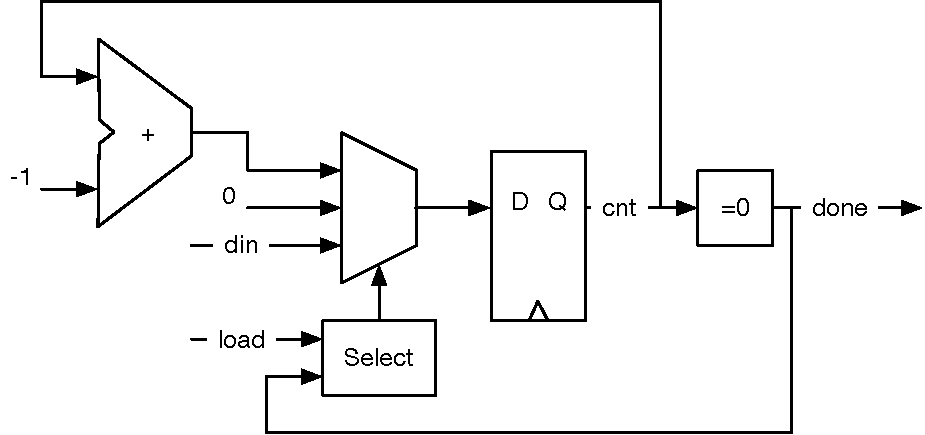
\includegraphics[scale=\scale]{../figures/timer}
\end{figure}
\end{frame}

\begin{frame}[fragile]{One-Shot Timer}
\shortlist{../code/timer.txt}
\end{frame}

\begin{frame}[fragile]{Summary on Counters}
\begin{itemize}
\item Counters are versatile tools
\item Count events
\item Generate timing ticks
\item Generate a one-shot timer
\end{itemize}
\end{frame}




\begin{frame}[fragile]{Add the following as new material to the repetition of the component/IO stuff}
\end{frame}

\begin{frame}[fragile]{Port Directions}
\begin{itemize}
\item Can be reversed with the \code{Flipped}
\item Convenient to have one bundle definition working as source
and destination used between two modules
\end{itemize}
\begin{chisel}
class Channel extends Bundle {
  val data = Input(UInt(32.W))
  val ready = Output(Bool())
  val valid = Input(Bool())
}

class ChannelUsage extends Bundle {
  val input = new Channel()
  val output = Flipped(new Channel())
}
\end{chisel}
\end{frame}

\begin{frame}[fragile]{Port Directions}
\begin{itemize}
\item Can be assigned at instantiation
\end{itemize}
\begin{chisel}
class ExecuteIO extends Bundle {
  val dec = Input(new DecodeExecute())
  val mem = Output(new ExecuteMemory())
}
\end{chisel}
\begin{chisel}
\end{chisel}
\end{frame}

\begin{frame}[fragile]{Connections}
\begin{itemize}
\item Simple connections just with assignments, e.g.,
\begin{chisel}
  adder.io.a := ina
  adder.io.b := inb
\end{chisel}
\item Automatic bulk connections between components
\begin{chisel}
  dec.io <> exe.io
  mem.io <> exe.io
\end{chisel}
\end{itemize}
\end{frame}





\begin{frame}[fragile]{Testing}
\begin{chisel}
class CounterTester(c: Counter) extends PeekPokeTester(c) {
  for (i <- 0 until 5) {
    println(i.toString + ": " + peek(c.io.out).toString())
    step(1)
  }
}
\end{chisel}
\begin{itemize}
\item Within Chisel with a tester (= Scala program)
\item May include waveform generation
\item peek and poke to read and set values
\begin{itemize}
\item Remember the BASIC days ;-)
\end{itemize}
\item printf in simulation on rising edge
\begin{chisel}
printf("Counting %x\n", r1)
\end{chisel}
\end{itemize}
\end{frame}



\begin{frame}[fragile]{Scala Build Tool (sbt)}
\begin{itemize}
\item Downloads Scala compiler if needed
\item Downloads dependent libraries (e.g., Chisel)
\item Compiles Scala programs
\item Executes Scala programs
\item Does a lot of magic, maybe too much
\item Compile and run with:
\end{itemize}
\begin{chisel}
sbt "runMain simple.Example"
\end{chisel}
\begin{itemize}
\item Or even just:
\end{itemize}
\begin{chisel}
sbt run
\end{chisel}
\end{frame}

\begin{frame}[fragile]{Build Configuration}
\begin{itemize}
\item Defines needed Scala version
\item Library dependencies
\item File name: \code{build.sbt}
\end{itemize}
\begin{chisel}
scalaVersion := "2.11.7"

resolvers ++= Seq(
  Resolver.sonatypeRepo("snapshots"),
  Resolver.sonatypeRepo("releases")
)

libraryDependencies += "edu.berkeley.cs" %% "chisel3" % "3.1.2"
libraryDependencies += "edu.berkeley.cs" %% "chisel-iotesters" % "1.2.2"
\end{chisel}
\end{frame}


\begin{frame}[fragile]{What is a Minimal Chisel Project?}
\begin{itemize}
\item Scala class (e.g., \code{Hello.scala})
\item Build info in \code{build.sbt} for \code{sbt}:
\end{itemize}
\begin{chisel}
scalaVersion := "2.11.7"

libraryDependencies += "edu.berkeley.cs" %% "chisel3" % "3.1.2"
\end{chisel}
\begin{itemize}
\item Run the process manually (look into the Makefile)
\end{itemize}
\end{frame}




\begin{frame}[fragile]{Chisel Main for Testing}
\begin{itemize}
\item Tests can be written in Scala/Chisel
\item Tester and device under test (DUT) are two processes
\item Invoke \code{execute} with some parameters, the DUT, and a tester
\end{itemize}
\begin{chisel}
object CounterTester extends App {

  iotesters.Driver.execute(Array[String](), () => new Counter(2)) {
    c => new CounterTester(c)
  }
}
\end{chisel}
\end{frame}

\begin{frame}[fragile]{A Chisel Tester}
\begin{itemize}
\item Extends class \code{PeekPokeTester}
\item Has the DUT as parameter
\item Testing code can use all features of Scala
\end{itemize}
\begin{chisel}
class CounterTester(dut: Counter) extends PeekPokeTester(dut) {

  // Here comes the Chisel/Scala code
  // for the testing
}
\end{chisel}
\end{frame}

\begin{frame}[fragile]{Testing}
\begin{itemize}
\item Set input values with \code{poke}
\item Advance the simulation with \code{step}
\item Read the output values with \code{peek}
\item Compare the values with \code{expect}
\end{itemize}
\end{frame}

\begin{frame}[fragile]{Testing Example}
\begin{chisel}
// Set input values
poke(dut.io.a, 3)
poke(dut.io.b, 4)
// Execute one iteration
step(1)
// Print the result
val res = peek(dut.io.result)
println(res)

// Or compare against expected value
expect(dut.io.result, 7)
\end{chisel}
\end{frame}


\begin{frame}[fragile]{Generating Wave Forms}
\begin{itemize}
\item Additional parameters: \code{"--generate-vcd-output", "on"}
\item IO signals and registers are dumped
\item Option \code{--debug} puts all wires into the dump
\item Generates a .vcd file
\item Viewing with gtkwave or ModelSim
\item See the example with \code{make fifo}
\begin{itemize}
\item Show it
\end{itemize}
\item BubbleFifo contains also longer testing code
\end{itemize}
\end{frame}


\begin{frame}[fragile]{Summary}
\begin{itemize}
\item TODO
\end{itemize}
\end{frame}


\end{document}

